	\section{Simulations}
	To demonstrate the previous results for the variance of $\hat{P}$ and Relative Efficiency (Equations x.x and x.x), we simulate random graphs from a SBM with parameters.
	\begin{equation*}
	B = \begin{bmatrix}
	.42 & .2 \\
	.2 & .7 
	\end{bmatrix}
	,\qquad \rho = \begin{bmatrix}
	.5 & .5
	\end{bmatrix}
	\end{equation*}
	
	From this model we sample $M$ adjacency matrices with $N$ vertices to calculate both $\bar{A}$ and $\hat{P}$.  With these estimators for $P$, we calculate the mean squared error of each block region in the model, defined as edges of the adjacency matrix that have the same edge-wise probability.  We then compare these simulations with our predictions.
	
	\begin{figure}[!htb]
		\centering
		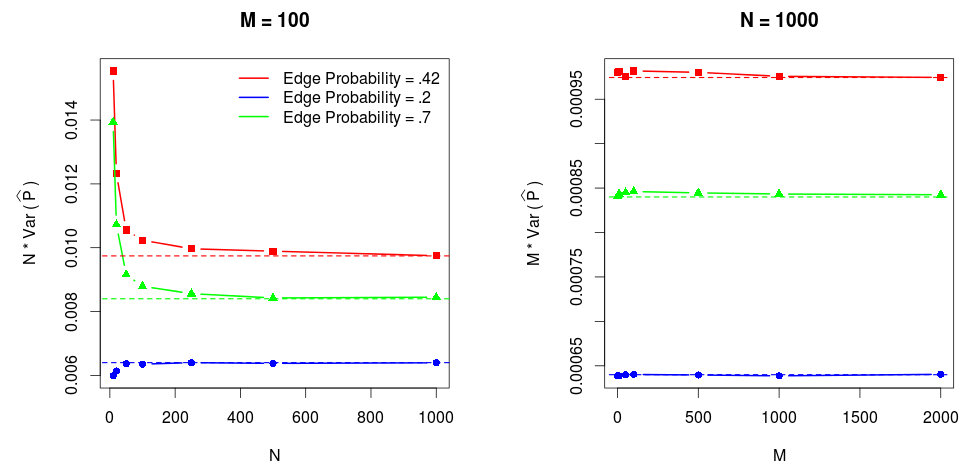
\includegraphics[width=16cm]{VarNM_rho.PNG}
		\caption{N*Var$(\hat{P})$ (a) and  M*Var$(\hat{P})$ (b) calculated from edges with associated edge probabilities, while increasing N and M, respectively.  Observe that the simulated values asymptotically converge to the predictions, represented by the dotted lines.}
		\label{fig:plot1}
	\end{figure}
	
	\begin{figure}[!htb]
		\centering
		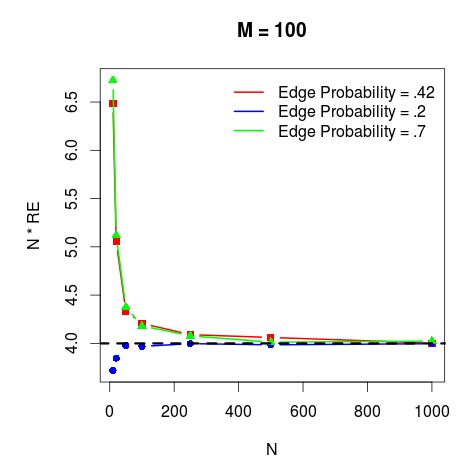
\includegraphics[width=9cm]{RE.PNG}
		\caption{N*RE calculated from edges with associated edge probabilities.  Observe that the simulated values asymptotically converge to the predictions, represented by the dotted line.}
		\label{fig:plot1}
	\end{figure}
	\newpage
	We now examine simulations where we vary the $\rho$ vector for the SBM with the following parameters:
	
		\begin{equation*}
		B = \begin{bmatrix}
		.42 & .2 \\
		.2 & .7 
		\end{bmatrix}
		,\qquad \rho = \begin{bmatrix}
			\rho_1 & \rho_2
		\end{bmatrix}
		,\qquad N = 500,\qquad M = 100
		\end{equation*}
	
	\begin{figure}[!htb]
		\centering
		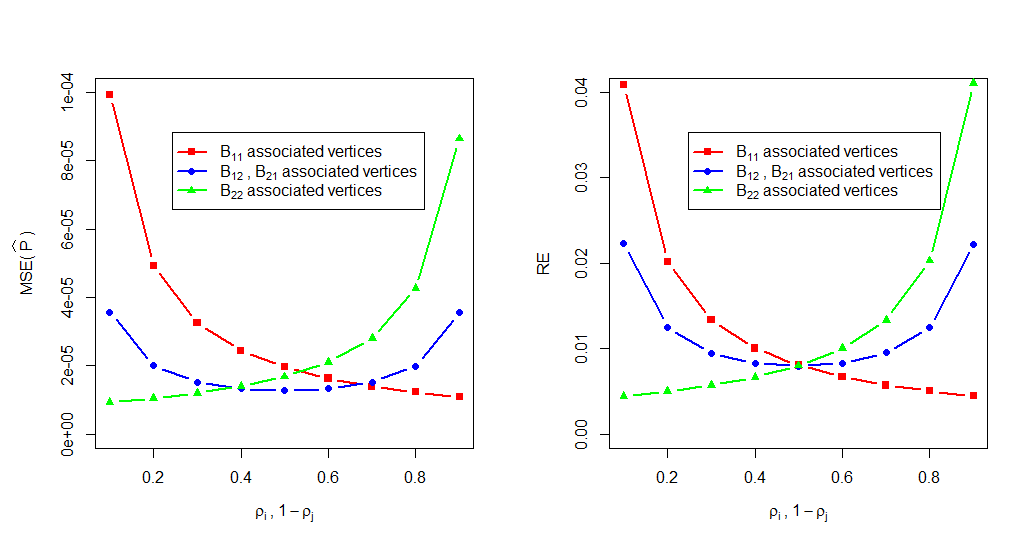
\includegraphics[width=16cm]{VarRE.PNG}
		\caption{Simulated results for Var$(\hat{P})$ (a) and RE (b) calculated from edges with associated edge probabilities. The simulated values for the variance and RE measurements deviated from the predictions with a mean of 3.7e-7, and 1.6e-4, respectively.}
		\label{fig:plot1}
	\end{figure}
	\newpage